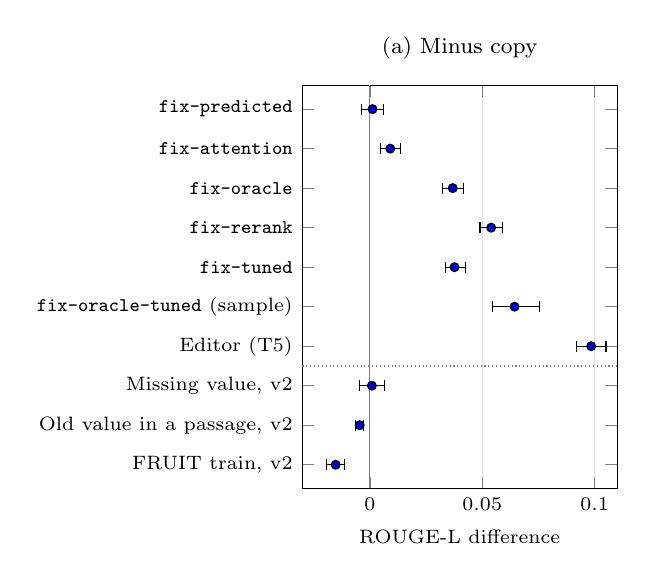
\begin{tikzpicture}
\begin{axis}[title={(a) Minus copy}, title style={font=\footnotesize}, width=0.46\linewidth, height=6.7cm,
  scale only axis=false, xmin=-0.03, xmax=0.11, ymin=-0.6, ymax=9.6,
  ytick={0,...,9}, yticklabels={{FRUIT train, v2},{Old value in a passage, v2},{Missing value, v2},{Editor (T5)},{\texttt{fix-oracle-tuned} (sample)},{\texttt{fix-tuned}},{\texttt{fix-rerank}},{\texttt{fix-oracle}},{\texttt{fix-attention}},{\texttt{fix-predicted}}}, yticklabel style={font=\scriptsize},
  xticklabel style={font=\scriptsize, /pgf/number format/fixed}, scaled x ticks=false,
  xlabel={ROUGE-L difference}, xlabel style={font=\scriptsize}, xmajorgrids, grid style={gray!25}]
\draw[gray] (axis cs:0,-0.6) -- (axis cs:0,9.6);
\draw[densely dotted, gray] (axis cs:-0.03,2.5) -- (axis cs:0.11,2.5);
\addplot+[only marks, mark=*, mark size=1.6pt, black, error bars/.cd, x dir=both, x explicit, error mark options={rotate=90, mark size=2pt}]
  coordinates {(-0.0152,0) += (0.0041,0) -= (0.0041,0) (-0.0045,1) += (0.0018,0) -= (0.0019,0) (0.0009,2) += (0.0056,0) -= (0.0055,0) (0.0985,3) += (0.0066,0) -= (0.0066,0) (0.0644,4) += (0.0110,0) -= (0.0099,0) (0.0377,5) += (0.0048,0) -= (0.0042,0) (0.0540,6) += (0.0051,0) -= (0.0050,0) (0.0369,7) += (0.0048,0) -= (0.0047,0) (0.0091,8) += (0.0047,0) -= (0.0043,0) (0.0012,9) += (0.0048,0) -= (0.0048,0)};
\end{axis}
\end{tikzpicture}\hfill
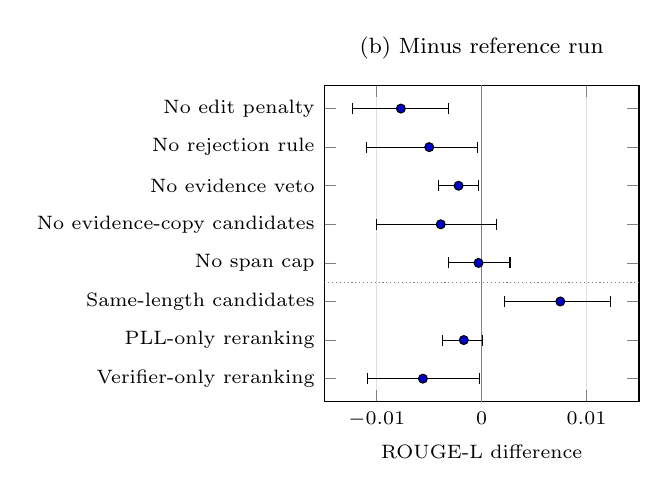
\begin{tikzpicture}
\begin{axis}[title={(b) Minus reference run}, title style={font=\footnotesize}, width=0.46\linewidth, height=5.60cm,
  scale only axis=false, xmin=-0.015, xmax=0.015, ymin=-0.6, ymax=7.6,
  ytick={0,...,7}, yticklabels={{Verifier-only reranking},{PLL-only reranking},{Same-length candidates},{No span cap},{No evidence-copy candidates},{No evidence veto},{No rejection rule},{No edit penalty}}, yticklabel style={font=\scriptsize},
  xticklabel style={font=\scriptsize, /pgf/number format/fixed}, scaled x ticks=false,
  xlabel={ROUGE-L difference}, xlabel style={font=\scriptsize}, xmajorgrids, grid style={gray!25}]
\draw[gray] (axis cs:0,-0.6) -- (axis cs:0,7.6);
\draw[densely dotted, gray] (axis cs:-0.015,2.5) -- (axis cs:0.015,2.5);
\addplot+[only marks, mark=*, mark size=1.6pt, black, error bars/.cd, x dir=both, x explicit, error mark options={rotate=90, mark size=2pt}]
  coordinates {(-0.0056,0) += (0.0054,0) -= (0.0053,0) (-0.0017,1) += (0.0018,0) -= (0.0020,0) (0.0075,2) += (0.0048,0) -= (0.0053,0) (-0.0003,3) += (0.0030,0) -= (0.0029,0) (-0.0039,4) += (0.0053,0) -= (0.0061,0) (-0.0022,5) += (0.0019,0) -= (0.0019,0) (-0.0050,6) += (0.0046,0) -= (0.0060,0) (-0.0077,7) += (0.0045,0) -= (0.0046,0)};
\end{axis}
\end{tikzpicture}
